\documentclass[11pt,a4paper]{article}
\usepackage[style=apa, backend=biber]{biblatex}
\usepackage[utf8]{inputenc}
\usepackage[ngerman]{babel}
\usepackage{csquotes}
\usepackage{hyperref}
\usepackage{tabularx}
\usepackage{calc}
\usepackage{geometry}
\usepackage[scaled]{helvet}
\usepackage[T1]{fontenc}
\usepackage{float}
\usepackage{graphicx}

% Bibliography
\addbibresource{references.bib}

\renewcommand{\familydefault}{\sfdefault}

\geometry{
  left=1.5cm,
  right=1.5cm,
  top=1.5cm,
  bottom=1.5cm,
  includeheadfoot
}

% Schriftgrössen und Titeldefinitionen
\newcommand{\titleformat}{\fontsize{18pt}{22pt}\selectfont}
\newcommand{\sectionformat}{\fontsize{14pt}{18pt}\selectfont}
\newcommand{\subsectionformat}{\fontsize{11pt}{14pt}\selectfont}
\newcommand{\bodytextformat}{\fontsize{10pt}{12pt}\selectfont}


\begin{document}

\begin{flushleft}
    {\titleformat\textbf{Integration einer Sprachsteuerungsfunktion in Mobile Apps}}\\[0.5cm]
  \end{flushleft}

\bodytextformat

\noindent
\begin{tabularx}{\linewidth}{@{}p{4cm}X@{}}
    \textbf{Themenbereiche:} & Sprachsteuerung, Audio, Machine Learning, Triggerwort-Erkennung, Mobile Apps \\
    \textbf{Studierender:} & Ruben Nuñez \\
    \textbf{Dozent:} & Dr. Florian Herzog \\
    \textbf{Experte:} & Damien Piguet \\
    \textbf{Auftraggeber:} & Stefan Reinhard \\
    \textbf{Keywords:} & Sprachsteuerung, Mobile Apps, Machine Learning, Triggerwort-Erkennung, Audioverarbeitung, Datensatzerstellung, Modelltraining, App-Integration \\
\end{tabularx}
    




\section{Aufgabenstellung}
Das Ziel dieser Bachelorarbeit ist die Entwicklung einer Sprachsteuerungsfunktion für mobile Anwendungen, mit einem besonderen Fokus auf der Erkennung von Triggerwörtern aus akustischer Sprache. Die Arbeit umfasst die Entwicklung eines Machine Learning-Modells, dessen Integration in eine mobile Plattform, insbesondere iOS, sowie die Berücksichtigung von Datenschutz und ethischen Richtlinien bei der Erstellung und Nutzung des für das Training des Modells erforderlichen Datensatzes.


\section{Ergebnisse}
Im Rahmen der Bachelorarbeit wurden folgende Ergebnisse erzielt:

\begin{itemize}
    \itemsep0em
    \item Ein \textbf{Machine Learning-Modell}, das in der Lage ist, Triggerwörter in akustischer Sprache zu erkennen.
    \item Eine \textbf{Integration in eine iOS-App}, die das Modell verwendet, um Triggerwörter in Echtzeit zu erkennen.
    \item Ein \textbf{Datensatz}, welcher ethische Richtlinien und Datenschutzbestimmungen einhält, wurde erstellt und verwendet, um das Modell zu trainieren.
    \item Eine \textbf{Dokumentation}, die die Entwicklung des Modells, die Erstellung des Datensatzes und die Implementierung der App beschreibt.
\end{itemize}

\noindent
Das Machine Learning Modell, benannt \textbf{WakeupTriggerConvLSTM2s}, ist eine Kombination aus einem \textit{Convolutional Neural Network} (CNN) und einem \textit{Long Short-Term Memory} (LSTM) Netzwerk. Das CNN extrahiert die akustischen Merkmale der Sprache, während das LSTM die zeitlichen Abhängigkeiten zwischen diesen Merkmalen erfasst. Es wurde in PyTorch implementiert, mit dem erstellten Datensatz trainiert und erreichte eine Genauigkeit (Accuracy) von 0.88 sowie einen F1-Score von 0.80 auf dem Testdatensatz. Zusätzlich wurde eine Transformationskomponente \textbf{AudioToSpectrogramTransformJit} in PyTorch entwickelt, die Audio in Spektrogramme umwandelt.

\noindent \newline
Die Effizienz des Modells, insbesondere im Hinblick auf Echtzeitfähigkeit, war entscheidend. Das Modell erreicht eine Vorhersagegeschwindigkeit von 0.01 Sekunden pro Spektrogramm, was den Anforderungen einer Echtzeiterkennung entspricht, ohne die Leistung des Geräts zu signifikant zu beeinträchtigen. Die entwickelten PyTorch-Module \textbf{AudioToSpectrogramTransformJit} und \textbf{WakeupTriggerConvLSTM2s} wurden in einer iOS-App implementiert, um eine effiziente Triggerworterkennung in Echtzeit zu ermöglichen.

\noindent \newline
Es wurde eine Recorder-Webseite für die Aufnahme von Sprachsamples entwickelt und auf der Google Cloud Platform gehostet. Diese Webseite ist eine dockerisierte Python Flask App die es ermöglichte eine effiziente Sammlung von Sprachdaten zu gewährleisten.

\noindent \newline
Zur Erhöhung der Diversität und Robustheit des Datensatzes kamen verschiedene Augmentierungstechniken zum Einsatz. Etwa 700 Sprachaufnahmen wurden von mehr als 10 Personen aufgenommen und durch Augmentierung auf 10.000 Samples erhöht. Der Datensatz beinhaltete neben dem Triggerwort 'Hey FOOBY' auch andere Wörter sowie Silence und Noise Samples, um das Modell unter verschiedenen Bedingungen zu trainieren und seine Reaktion auf Hintergrundgeräusche zu verbessern.


\newpage
\section{Lösungskonzept}
In dieser Bachelorarbeit wurde innerhalb von 14 Wochen ein System zur Erkennung von Triggerwörtern in akustischer Sprache entwickelt. Ein zentraler Bestandteil des Systems ist die Analyse von Audio-Chunks, um Triggerwörter zu identifizieren. Dafür wird in Echtzeit der Buffer des Mikrofons ausgelesen und in Audio-Chunks verarbeitet. Der Buffer ist so konfiguriert, dass er in einem Intervall von 0.1 Sekunden ausgelesen wird. Die Grösse der Audio-Chunks beträgt dabei 2 Sekunden, das entspricht 32000 Samples bei einer Samplerate von 16kHz. Die nachstehende Abbildung visualisiert die Struktur dieser Lösung.

\begin{figure}[H]
\centering
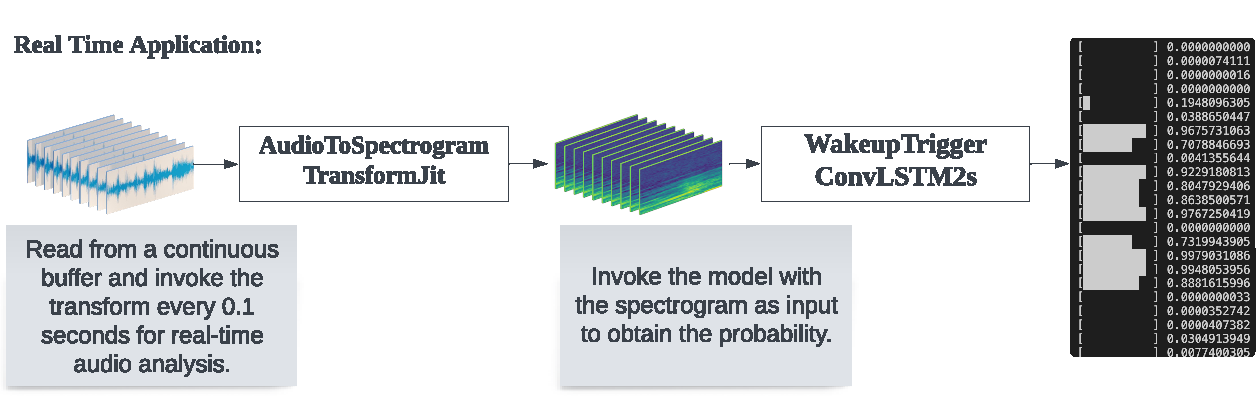
\includegraphics[width=1.0\linewidth, trim=0pt 10pt 0pt 15pt, clip]{img/realtime-application.pdf}
\caption{Schematische Darstellung der Real Time Anwendung}
\end{figure}

\noindent
Die Erkennung basiert auf der Berechnung des gleitenden Durchschnitts (SMA) der Wahrscheinlichkeiten der letzten n Audio-Chunks. Überschreitet der Durchschnitt einen festgelegten Schwellenwert, wird das Triggerwort als erkannt betrachtet. Diese Methode sichert eine effiziente und präzise Erkennung. Die folgende Abbildung illustriert die Berechnung des SMA für verschiedene Anzahlen von Audio-Chunks.

\begin{figure}[H]
\centering
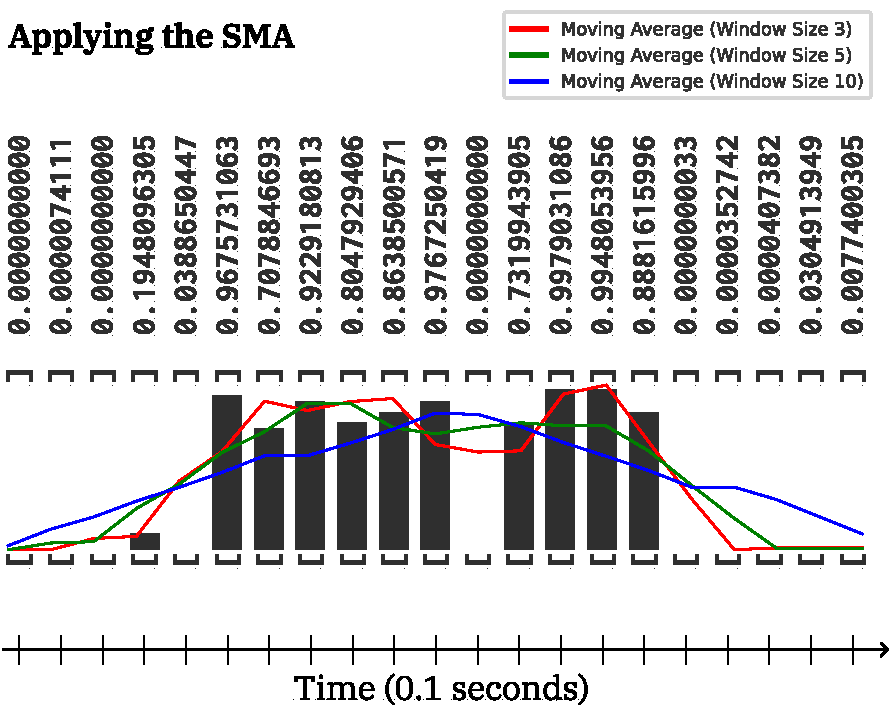
\includegraphics[width=.5\linewidth]{img/sma.pdf}
\caption{Darstellung der SMA-Berechnung über Audio-Chunks}
\end{figure}

\noindent
Durch die Kalibrierung des Schwellenwerts sowie der Anzahl Audio-Chunks, die für die Berechnung des SMA verwendet werden, kann die Sensitivität der Erkennung angepasst werden.

\noindent \newline
Ebenfalls wurden User Tests durchgeführt, um die Benutzerfreundlichkeit der App zu testen. Sechs Personen nahmen an den Tests teil. Bei den Tests wurde in einer Konfusionsmatrix die Anzahl der korrekten und falschen Erkennungen der Triggerwörter aufgezeichnet. Die Tests zeigten, dass die Erkennung des Triggerworts in 50 von 61 Fällen erkannt wurde (True Positive). In 11 von 61 Fällen wurde das Triggerwort nicht erkannt (False Negative). Bei der other Klasse wurden fälschlicherweise 28 von 63 Samples als Triggerwort erkannt (False Positive) und 35 von 63 Samples korrekt als other Klasse erkannt (True Negative). Die Konfusionsmatrix ist in der folgenden Abbildung dargestellt.

\begin{figure}[H]
\centering
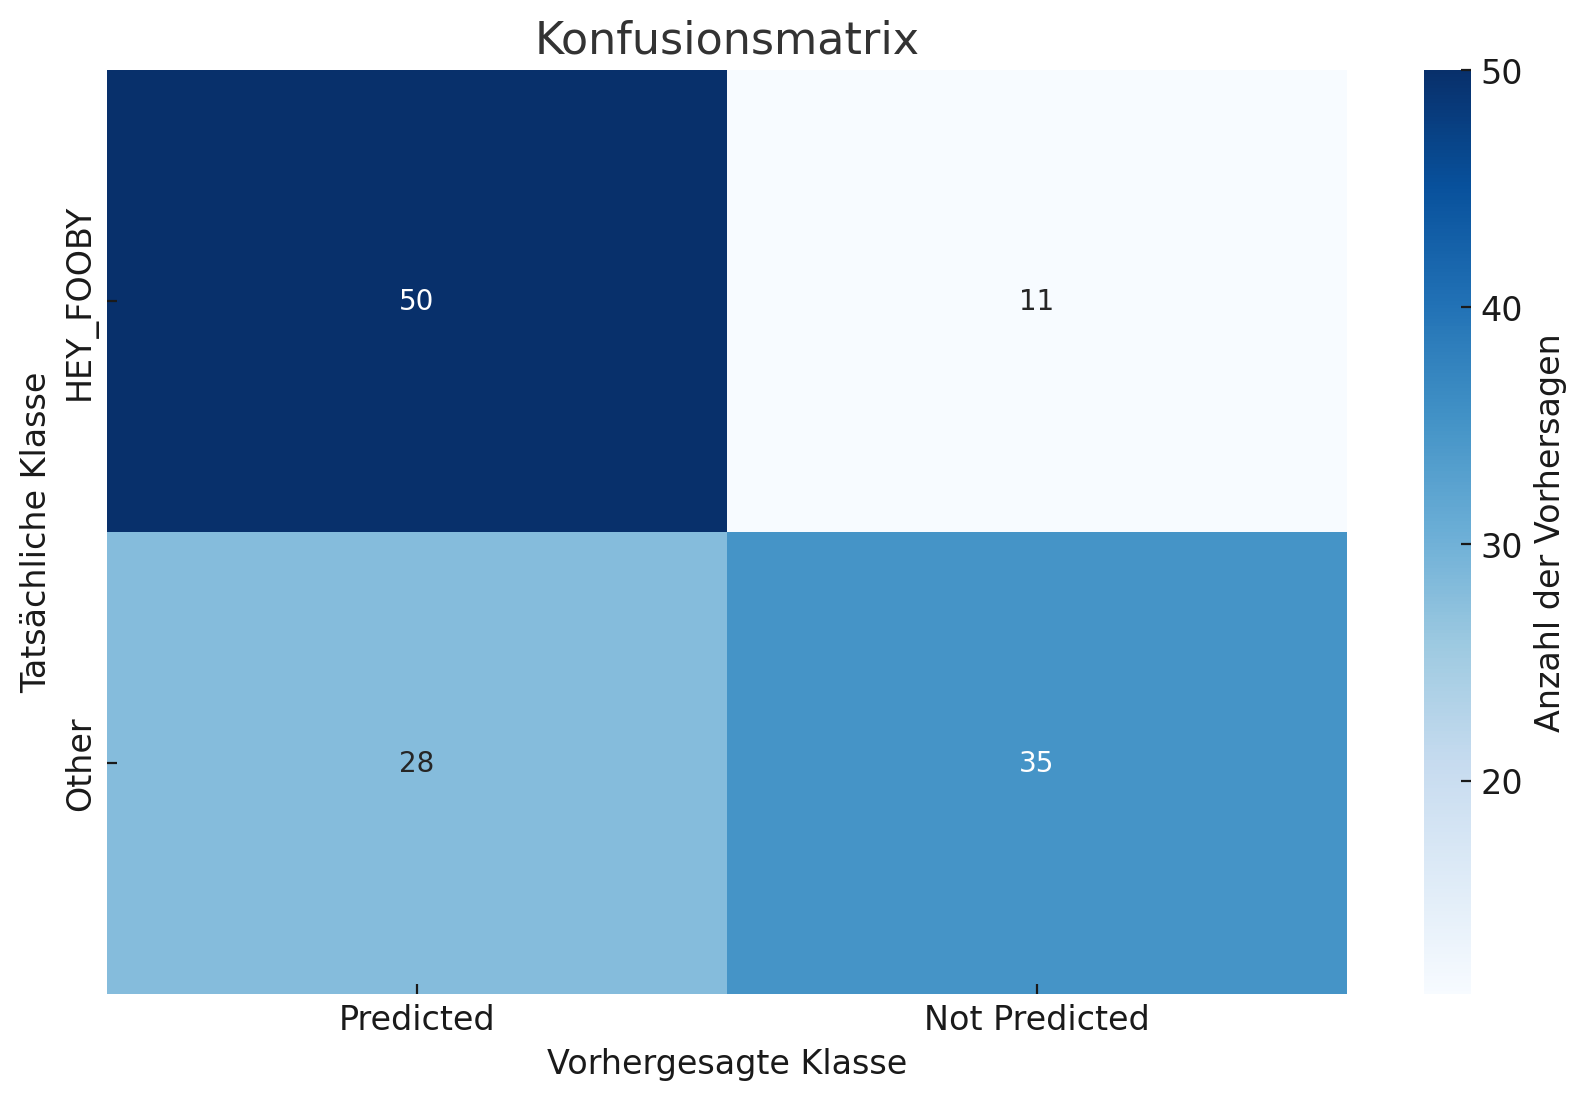
\includegraphics[width=.5\linewidth]{img/eval-usertests.png}
\caption{Konfusionsmatrix der User Tests}
\end{figure}


\section{Spezielle Herausforderungen}
Eines der Herausforderungen war es die erarbeiteten PyTorch Module über TorchScript zu konvertieren so dass diese in der iOS App verwendet werden können. Die Grundidee hinter TorchScript ist es, die PyTorch Module in ein Format zu konvertieren, das von der C++ API von PyTorch verwendet werden kann. 

\begin{displayquote}
TorchScript is a way to create serializable and optimizable models from PyTorch code. Any TorchScript program can be saved from a Python process and loaded in a process where there is no Python dependency. (\cite{pytorch2023jit})
\end{displayquote}

\noindent
Neben dem konvertieren musste auch die Integration in Objective-C, C++ und Swift erfolgen. Das Ganze ist dabei nicht so einfach wie es klingt. Es mussten einige Hürden überwunden werden, um die Module erfolgreich in die iOS App zu integrieren. Das Grundsätzliche Problem war, die fehlende Erfahrung in der Entwicklung mit Objective-C und C++.

\section{Ausblick}



\end{document}
